\subsection{物理法則から状態方程式を構成する手順}

状態方程式は、物理法則を行列記法へ置き換えただけのものではない。保存される量、流れとして入る量、素子や機構の構成則、入力と出力の選び方を順に固定し、将来の変化を一階微分方程式として計算できる形に整理したものである。集中定数モデルで最初に作る形は
\begin{align}
  \dot{x}(t)&=f(x(t),u(t),d(t),p,t),\\
  y(t)&=g(x(t),u(t),d(t),p,t)
\end{align}
である。線形時不変に近似できる場合は
\begin{align}
  \dot{x}(t)&=Ax(t)+Bu(t)+Ed(t),\label{eq:physical-modeling-state-form}\\
  y(t)&=C_y x(t)+D_y u(t)+F_y d(t)
\end{align}
と書く。ここで $C_y$ は出力行列であり、電気容量を表す $C$ と混同しないように添字を付けている。

\begin{definition}[構成則]
保存則や運動方程式だけでは、流れ、力、電圧、温度差の関係は決まらない。熱流と温度差、電流と電圧差、ばね力と変位、粘性力と速度のように、対象を構成する要素ごとの関係式を構成則という。
\end{definition}

物理モデルを状態方程式にする手順は、次の形にそろえられる。

\begin{enumerate}
  \item 蓄積される量を決める。熱なら内部エネルギー、電気なら電荷、機械なら運動量とばねの変位に相当する量である。
  \item 保存則または運動方程式を書く。蓄積量の時間変化率は、流入、流出、生成、外乱の和で決まる。
  \item 構成則で未知の流れや力を状態、入力、外乱、パラメータで表す。
  \item 入力 $u$、外乱 $d$、出力 $y$ を単位つきで選ぶ。
  \item 将来計算に必要な最小限の量を状態 $x$ とし、すべてを $\dot{x}=f(x,u,d,p,t)$ の形へ解く。二階微分が出る場合は、速度を新しい状態にして一階の連立方程式へ直す。
\end{enumerate}

この手順では、状態を「測れる量」として選ぶのではなく、「以後の変化を計算するのに必要な量」として選ぶ。測れる量は出力 $y$ に置く。状態を選んだ後で出力方程式を作ると、測定できる量と内部に保持すべき量を分けられる。

図\ref{fig:physical-modeling-examples} は、以後の導出で使う標準例を、蓄積要素、入力、外乱、出力の位置として並べたものである。熱系と RC 回路は一つの蓄積要素から一次モデルになり、質量ばねダンパ系と DC モータは速度、電流、角速度のような内部量を状態として残すことで一階の連立方程式になる。図の矢印は信号の向きだけでなく、式の右辺で正負どちらに入るかを確認するための手掛かりでもある。

\begin{figure}[tb]
\centering
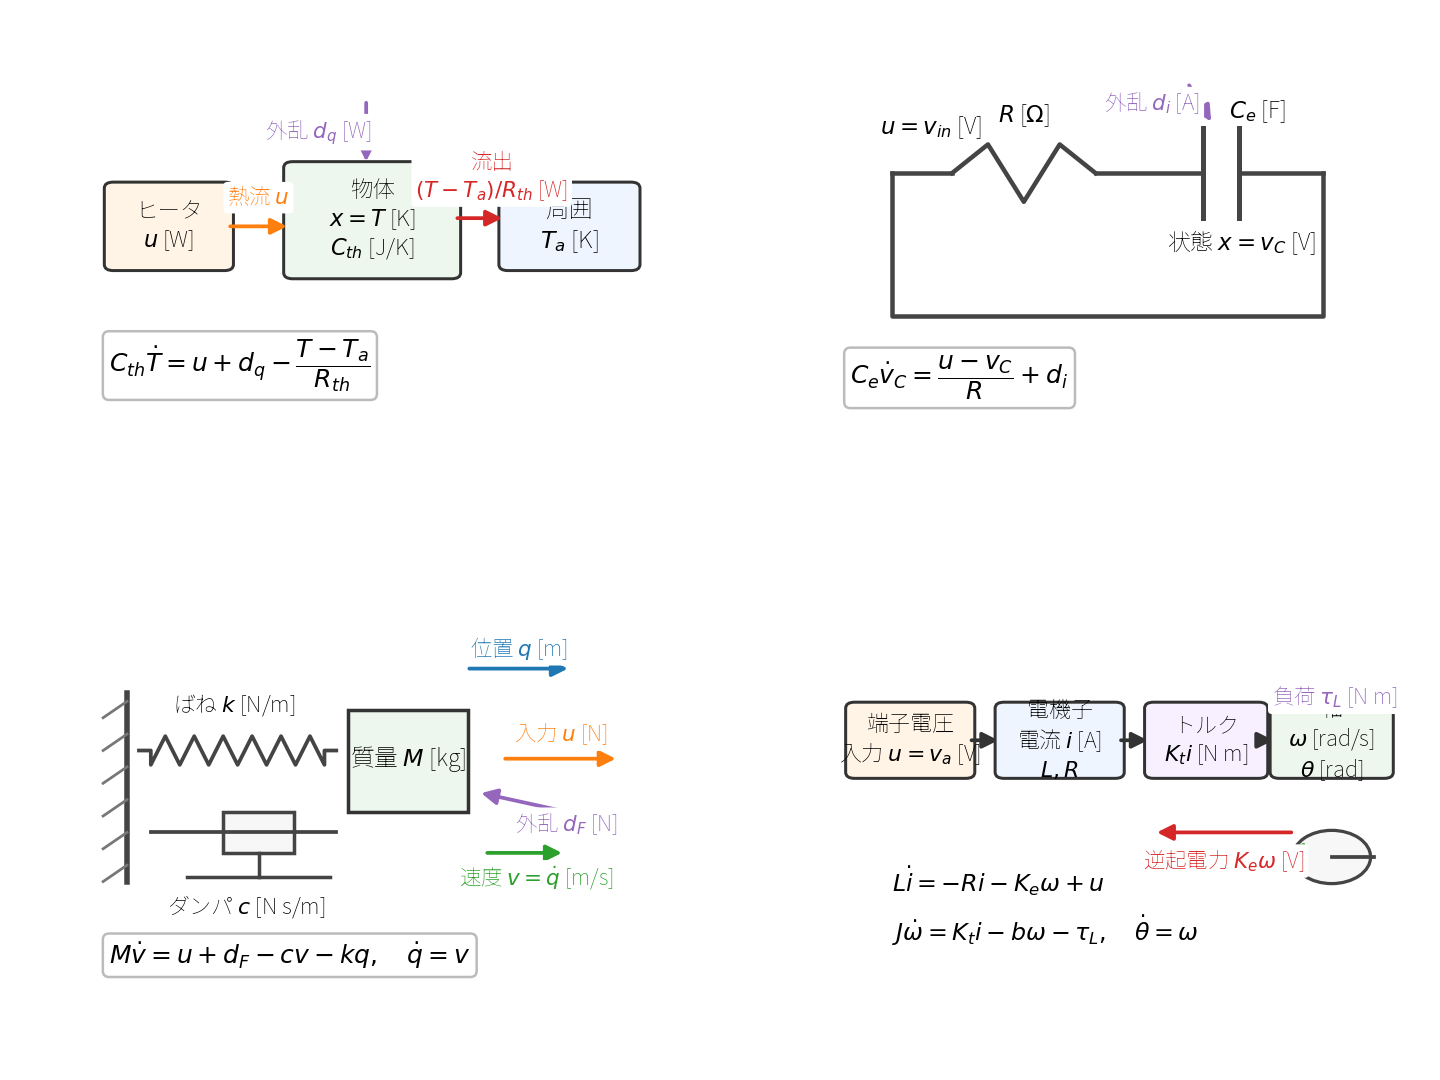
\includegraphics[width=0.96\linewidth,bb=0 0 1440 1080]{figures/physical_modeling_examples.png}
\caption{物理法則から状態方程式へ進む標準例。熱収支では内部エネルギーの蓄積、RC 回路では電荷の蓄積、質量ばねダンパ系では位置と速度、DC モータでは電流、角速度、角度を状態として残す。各パネルは入力、外乱、代表パラメータ、状態の単位を対応させ、保存則または運動方程式から $\dot{x}=f(x,u,d,p)$ へ整理する起点を示している。}
\label{fig:physical-modeling-examples}
\end{figure}

\begin{practice}[物理モデルの構造分類]
図\ref{fig:physical-modeling-examples} の四つの例について、蓄積される量、状態、入力、外乱、出力候補を一つずつ表にせよ。次に、熱系と RC 回路の式を見比べ、$C_{\mathrm{th}}$ と $C_e$、$R_{\mathrm{th}}$ と $R$、$T$ と $v_C$ がそれぞれどの役割に対応するかを説明せよ。最後に、質量ばねダンパ系で位置 $q$ だけを状態にした場合に未来の計算で不足する量を答えよ。
\end{practice}

\subsubsection{熱系の収支式からの導出}

一つの代表温度で表せる小さな物体を考える。温度を $T(t)$ [K]、周囲温度を $T_a(t)$ [K]、ヒータ熱流を $u(t)$ [W]、未知の熱流外乱を $d_q(t)$ [W] とする。熱容量を $C_{\mathrm{th}}$ [J/K]、熱抵抗を $R_{\mathrm{th}}$ [K/W] とし、物体内部の温度分布は無視できると仮定する。

蓄積される量は内部エネルギーであり、基準エネルギーを除けば変化率は
\begin{equation}
  \dot{E}(t)=C_{\mathrm{th}}\dot{T}(t)
\end{equation}
と書ける。単位は $(\mathrm{J/K})(\mathrm{K/s})=\mathrm{J/s}=\mathrm{W}$ であり、熱流と一致する。熱抵抗の構成則により、物体から周囲へ出る熱流は
\begin{equation}
  q_{\mathrm{out}}(t)=\frac{T(t)-T_a(t)}{R_{\mathrm{th}}}
\end{equation}
である。したがって熱収支は
\begin{align}
  C_{\mathrm{th}}\dot{T}(t)
  &=u(t)+d_q(t)-q_{\mathrm{out}}(t)\\
  &=u(t)+d_q(t)-\frac{T(t)-T_a(t)}{R_{\mathrm{th}}}
\end{align}
となる。状態を $x=T$、入力を $u$、外乱を
\begin{equation}
  d(t)=\begin{bmatrix}T_a(t)\\ d_q(t)\end{bmatrix}
\end{equation}
と選ぶと、一階の状態方程式は
\begin{equation}
  \dot{x}(t)
  =-\frac{1}{R_{\mathrm{th}}C_{\mathrm{th}}}x(t)
   +\frac{1}{C_{\mathrm{th}}}u(t)
   +\begin{bmatrix}
      \dfrac{1}{R_{\mathrm{th}}C_{\mathrm{th}}}&
      \dfrac{1}{C_{\mathrm{th}}}
    \end{bmatrix}d(t)
\end{equation}
である。出力として温度を測るなら
\begin{equation}
  y(t)=x(t)
\end{equation}
でよい。行列表示では $A=-1/(R_{\mathrm{th}}C_{\mathrm{th}})$、$B=1/C_{\mathrm{th}}$ であり、$A$ の単位は 1/s、$B$ の単位は K/J である。$B u$ の単位は $(\mathrm{K/J})(\mathrm{J/s})=\mathrm{K/s}$ となり、$\dot{x}$ の単位と一致する。

\subsubsection{RC 回路のキルヒホッフ則からの導出}

抵抗とコンデンサからなる一次の RC 回路を考える。入力電圧を $u(t)=v_{\mathrm{in}}(t)$ [V]、コンデンサ電圧を $v_C(t)$ [V]、節点へ流れ込む未知電流を $d_i(t)$ [A] とする。抵抗を $R$ [$\Omega$]、容量を $C_e$ [F] とし、抵抗と容量は一定、配線の寄生成分は無視できると仮定する。

蓄積される量はコンデンサの電荷
\begin{equation}
  Q_C(t)=C_e v_C(t)
\end{equation}
である。電荷の時間変化率は電流なので
\begin{equation}
  \dot{Q}_C(t)=C_e\dot{v}_C(t)
\end{equation}
であり、単位は $\mathrm{C/s}=\mathrm{A}$ である。抵抗を流れてコンデンサ節点へ入る電流は、オームの法則により
\begin{equation}
  i_R(t)=\frac{u(t)-v_C(t)}{R}
\end{equation}
である。キルヒホッフの電流則を節点に適用すると、コンデンサへ流れ込む電流の和が電荷の増加率になるため
\begin{align}
  C_e\dot{v}_C(t)&=i_R(t)+d_i(t)\\
  &=\frac{u(t)-v_C(t)}{R}+d_i(t)
\end{align}
を得る。状態を $x=v_C$、入力を $u=v_{\mathrm{in}}$、外乱を $d=d_i$ と置けば
\begin{align}
  \dot{x}(t)&=-\frac{1}{RC_e}x(t)+\frac{1}{RC_e}u(t)+\frac{1}{C_e}d(t),\\
  y(t)&=x(t)
\end{align}
である。このモデルでは $A=-1/(RC_e)$、$B=1/(RC_e)$ であり、どちらも 1/s の単位をもつ。電流外乱の係数 $1/C_e$ は、電流 [A] を電圧変化率 [V/s] に変える係数である。熱系と RC 回路の式が同じ形になるのは、熱容量とコンデンサ容量が蓄積を表し、熱抵抗と電気抵抗が差に比例する流れを作るからである。

\subsubsection{質量ばねダンパ系の運動方程式からの導出}

水平直線上の質量を考える。位置を $q(t)$ [m]、速度を $v(t)=\dot{q}(t)$ [m/s]、入力として加える力を $u(t)$ [N]、外力外乱を $d_F(t)$ [N] とする。質量を $M$ [kg]、粘性係数を $c$ [N\,s/m]、ばね定数を $k$ [N/m] とし、ばねの自然長からの変位を $q=0$ 基準で測る。

機械系では、力のつり合いではなくニュートンの第二法則を使う。運動量 $Mv$ の時間変化率が力の和であるから
\begin{equation}
  M\dot{v}(t)=\sum F(t)
\end{equation}
である。ばね力と粘性力の構成則を
\begin{equation}
  F_k(t)=-kq(t),\qquad F_c(t)=-cv(t)
\end{equation}
と置くと
\begin{align}
  M\dot{v}(t)&=u(t)+d_F(t)-cv(t)-kq(t),\\
  \dot{q}(t)&=v(t)
\end{align}
を得る。二階微分方程式としては
\begin{equation}
  M\ddot{q}(t)+c\dot{q}(t)+kq(t)=u(t)+d_F(t)
\end{equation}
であるが、状態方程式では一階の連立方程式に直す。状態を
\begin{equation}
  x(t)=\begin{bmatrix}q(t)\\ v(t)\end{bmatrix}
\end{equation}
と選ぶと
\begin{align}
  \dot{x}(t)
  &=\begin{bmatrix}
      0&1\\
      -k/M&-c/M
    \end{bmatrix}x(t)
    +\begin{bmatrix}
      0\\
      1/M
    \end{bmatrix}u(t)
    +\begin{bmatrix}
      0\\
      1/M
    \end{bmatrix}d_F(t),\label{eq:physical-modeling-msd-state}\\
  y(t)&=\begin{bmatrix}1&0\end{bmatrix}x(t)
\end{align}
となる。位置だけを測る場合は出力行列が $\begin{bmatrix}1&0\end{bmatrix}$ であり、速度まで測る場合は $y=x$ としてよい。\weq{physical-modeling-msd-state} の $A_{21}=-k/M$ は 1/s$^2$、$A_{22}=-c/M$ は 1/s、$B_2=1/M$ は 1/kg の単位をもつ。状態の成分 $q$ と $v$ の単位が異なるため、状態行列の各成分の単位も異なる。

熱系と RC 回路では一つの蓄積要素から一つの状態が生じた。質量ばねダンパ系では、位置だけでは次の位置を計算できず、速度も必要になる。したがって状態は $q$ だけでなく $v$ を含む。この違いは、モデルの次数が「式の見た目」ではなく、蓄積要素と将来計算に必要な情報の数で決まることを示している。

\subsubsection{DC モータの電気機械結合モデルの導出}

直流モータは、電気回路と回転運動が結合した標準的な制御対象である。ここでは電機子制御の DC モータを考え、端子電圧を $u(t)=v_a(t)$ [V]、電機子電流を $i(t)$ [A]、回転角を $\theta(t)$ [rad]、角速度を $\omega(t)=\dot{\theta}(t)$ [rad/s]、負荷トルクを $\tau_L(t)$ [N\,m] とする。電機子インダクタンスを $L$ [H]、電機子抵抗を $R$ [$\Omega$]、逆起電力定数を $K_e$ [V\,s/rad]、トルク定数を $K_t$ [N\,m/A]、回転部の等価慣性モーメントを $J$ [kg\,m$^2$]、粘性摩擦係数を $b$ [N\,m\,s/rad] とする。磁束は一定、磁気飽和、ブラシ電圧降下、クーロン摩擦、軸のねじれは無視し、すべてのパラメータは一定と仮定する。

電気側ではキルヒホッフの電圧則を使う。電機子端子に加えた電圧は、インダクタンスの電圧降下、抵抗の電圧降下、回転によって生じる逆起電力の和である。構成則を
\begin{equation}
  v_L(t)=L\dot{i}(t),\qquad
  v_R(t)=Ri(t),\qquad
  e_b(t)=K_e\omega(t)
\end{equation}
と置くと
\begin{equation}
  u(t)=L\dot{i}(t)+Ri(t)+K_e\omega(t)
\end{equation}
である。したがって電流の状態方程式は
\begin{equation}
  \dot{i}(t)=-\frac{R}{L}i(t)-\frac{K_e}{L}\omega(t)+\frac{1}{L}u(t)
  \label{eq:dcmotor-current-state}
\end{equation}
となる。各項の単位は A/s でそろう。たとえば $R i/L$ は V/H であり、$1\,\mathrm{H}=1\,\mathrm{V\,s/A}$ だから A/s である。

機械側では、回転に関するニュートンの第二法則を使う。角運動量 $J\omega$ の時間変化率は、軸まわりのトルクの和である。モータが作るトルクと粘性摩擦トルクを
\begin{equation}
  \tau_m(t)=K_t i(t),\qquad
  \tau_b(t)=b\omega(t)
\end{equation}
と置けば
\begin{equation}
  J\dot{\omega}(t)=K_t i(t)-b\omega(t)-\tau_L(t)
\end{equation}
であり、
\begin{equation}
  \dot{\omega}(t)=\frac{K_t}{J}i(t)-\frac{b}{J}\omega(t)-\frac{1}{J}\tau_L(t)
  \label{eq:dcmotor-speed-state}
\end{equation}
を得る。さらに角度は角速度の積分で決まるため
\begin{equation}
  \dot{\theta}(t)=\omega(t)
  \label{eq:dcmotor-angle-state}
\end{equation}
である。

角度制御まで含めるなら、状態を
\begin{equation}
  x(t)=\begin{bmatrix}i(t)\\ \omega(t)\\ \theta(t)\end{bmatrix},
  \qquad d(t)=\tau_L(t)
\end{equation}
と選ぶ。\weq{dcmotor-current-state}--\weq{dcmotor-angle-state} をまとめると
\begin{align}
  \dot{x}(t)
  &=
  \begin{bmatrix}
    -R/L&-K_e/L&0\\
    K_t/J&-b/J&0\\
    0&1&0
  \end{bmatrix}x(t)
  +\begin{bmatrix}
    1/L\\
    0\\
    0
  \end{bmatrix}u(t)
  +\begin{bmatrix}
    0\\
    -1/J\\
    0
  \end{bmatrix}d(t),\label{eq:dcmotor-state-space}\\
  y(t)&=C_y x(t)+D_y u(t)
\end{align}
となる。角速度を測って速度制御をする場合は $C_y=\begin{bmatrix}0&1&0\end{bmatrix}$、$D_y=0$ と置く。角度エンコーダで位置制御をする場合は $C_y=\begin{bmatrix}0&0&1\end{bmatrix}$ である。電流センサとエンコーダの両方を使うなら
\begin{equation}
  y(t)=
  \begin{bmatrix}
    1&0&0\\
    0&0&1
  \end{bmatrix}x(t)
\end{equation}
のように出力を複数にしてよい。

パラメータの意味は、応答の速さと結合の強さに直接現れる。$L/R$ は電気的時定数であり、回転が止まっていて逆起電力がないときの電流の立ち上がりを決める。$J/b$ は、電流を 0 として粘性摩擦だけで減速するときの機械的時定数である。$K_e$ が大きいほど同じ角速度で大きな逆起電力が生じ、電流の増加を抑える。$K_t$ が大きいほど同じ電流で大きなトルクが得られる。SI 単位系で同じ物理変換を理想的に表すと $K_t$ と $K_e$ の数値は一致するが、制御モデルでは単位と符号の定義を明示してから使う必要がある。負荷トルク $\tau_L$ は入力電圧で直接選べないため外乱として置き、速度低下や位置誤差を通じて観測される。

速度制御だけが目的で、角度 $\theta$ が出力にも制約にも入らない場合は、状態を $x=[i,\omega]^\T$ に縮約できる。一方、電気的時定数 $L/R$ が制御周期や機械応答に比べて十分小さい場合は、近似的に $L\dot{i}\simeq0$ と置き
\begin{equation}
  i(t)\simeq\frac{u(t)-K_e\omega(t)}{R}
\end{equation}
として、電流状態を消去する低次モデルを作ることもある。この近似は電流制御器が内側で十分速く働く場合にも使われる。ただし電流制限や過渡的なトルク応答を評価する設計では、\weq{dcmotor-state-space} のように電流を状態として残す方が適切である。

熱、電気、並進機械、回転機械の四例だけでは、保存則が流量で決まる対象と、重力で非線形な復元力を受ける対象をまだ十分に分けられない。水位制御では、センサが水位を測り、ポンプや弁が流量を変える。振子では、角度を測り、支点トルクで姿勢を変える。どちらも低次の制御対象として扱えるが、タンクでは流出量が水位の平方根に依存し、振子では重力項が $\sin\theta$ に依存する。図\ref{fig:tank-pendulum-modeling-examples} は、この二つの対象で、蓄積量、構成則、局所近似、パラメータ変化を対応させたものである。

\begin{figure}[tb]
\centering
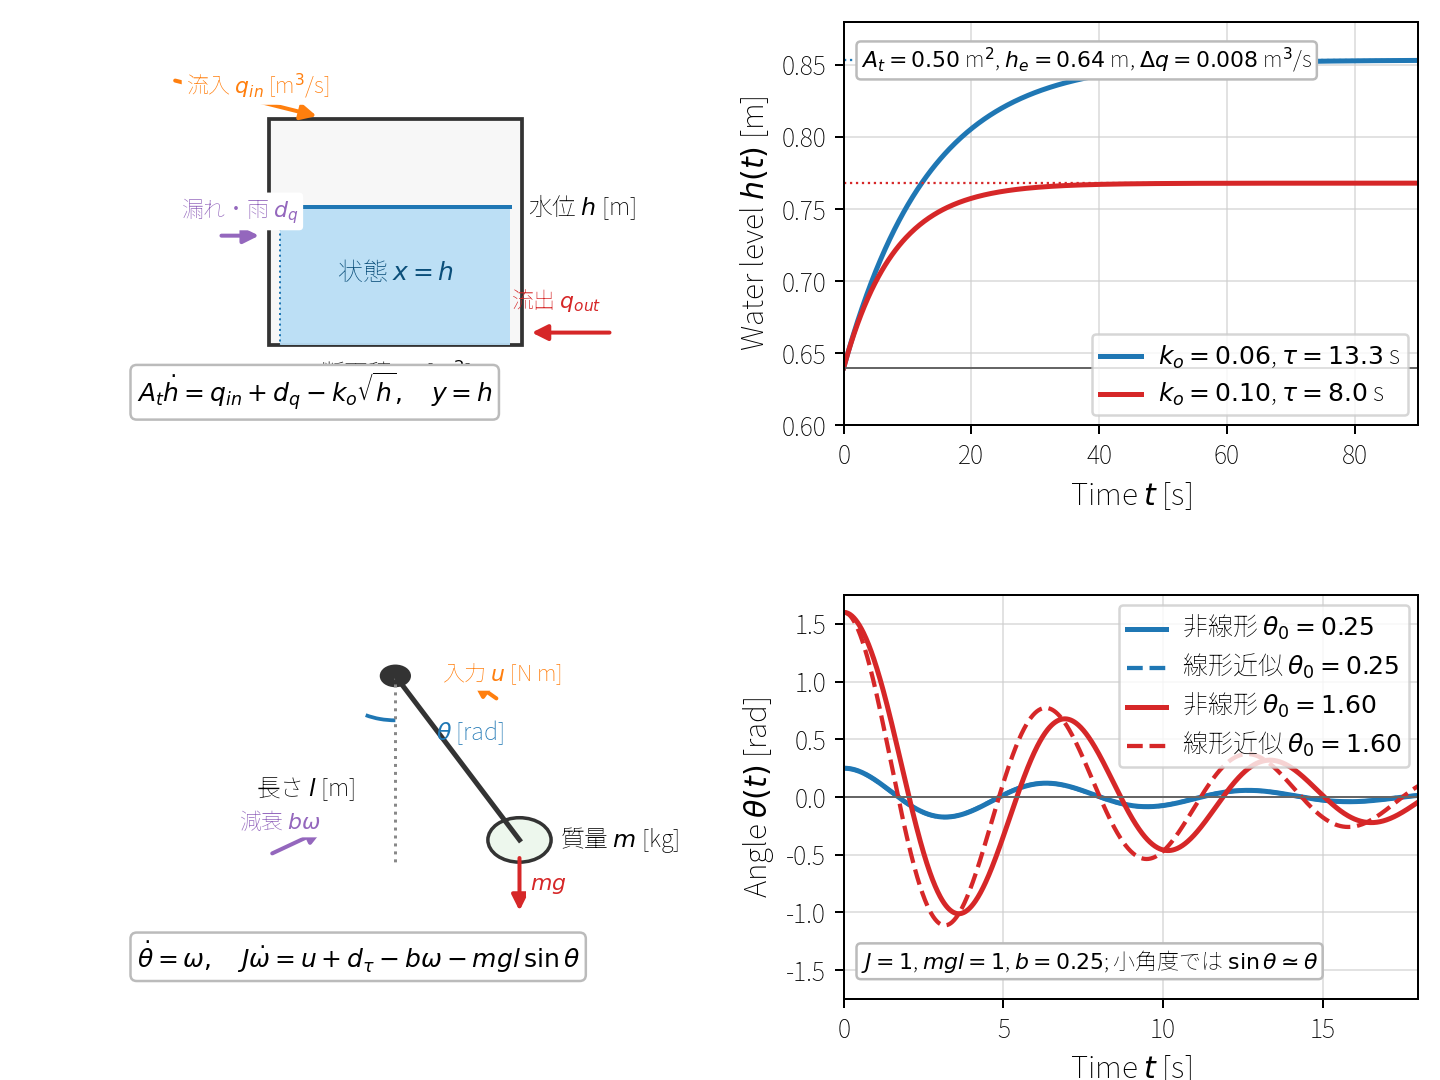
\includegraphics[width=0.96\linewidth,bb=0 0 1440 1080]{figures/tank_pendulum_modeling_examples.png}
\caption{タンク水位モデルと単振子モデルの構造。タンクでは体積保存則と流出構成則から水位の状態方程式が得られ、流出係数 $k_o$ を変えると線形化後の時定数と定常水位変化が同時に変わる。単振子ではトルク、重力、粘性減衰から角度と角速度の状態方程式が得られ、小角度では線形近似と非線形応答が一致しやすいが、大振幅では周期と振幅がずれる。}
\label{fig:tank-pendulum-modeling-examples}
\end{figure}

\subsubsection{単一タンクの水位状態方程式}

断面積が一定のタンクを考える。水位を $h(t)$ [m]、断面積を $A_t$ [m$^2$]、ポンプ流入を $q_{\mathrm{in}}(t)$ [m$^3$/s]、雨や漏れをまとめた流量外乱を $d_q(t)$ [m$^3$/s] とする。出力は水位センサで測る $y(t)=h(t)$ とする。タンク内の水量は体積
\begin{equation}
  V(t)=A_t h(t)
\end{equation}
であり、体積の時間変化率は流入から流出を引いた正味流量で決まる。

底の小さな出口から大気中へ流れる場合、流速は水位差によって変わる。ここでは出口断面積、流量係数、重力加速度をまとめた係数 $k_o$ を用いて
\begin{equation}
  q_{\mathrm{out}}(t)=k_o\sqrt{h(t)},\qquad h(t)\ge0
\end{equation}
と書く。$q_{\mathrm{out}}$ の単位は m$^3$/s なので、$k_o$ の単位は m$^{5/2}$/s である。したがって保存則は
\begin{align}
  \frac{\dd}{\dd t}\{A_t h(t)\}
  &=q_{\mathrm{in}}(t)+d_q(t)-q_{\mathrm{out}}(t)\\
  A_t\dot{h}(t)
  &=q_{\mathrm{in}}(t)+d_q(t)-k_o\sqrt{h(t)}
\end{align}
となる。状態を $x=h$ と選べば、非線形状態方程式は
\begin{align}
  \dot{x}(t)&=\frac{1}{A_t}\{q_{\mathrm{in}}(t)+d_q(t)-k_o\sqrt{x(t)}\},\label{eq:tank-level-state}\\
  y(t)&=x(t)
\end{align}
である。

一定流入 $q_{\mathrm{in},e}$ と一定外乱 $d_{q,e}$ のもとで水位 $h_e>0$ が保たれるには
\begin{equation}
  q_{\mathrm{in},e}+d_{q,e}=k_o\sqrt{h_e}
  \label{eq:tank-level-equilibrium}
\end{equation}
が必要である。この平衡点の近くで
\begin{equation}
  \tilde{h}=h-h_e,\qquad
  \tilde{q}_{\mathrm{in}}=q_{\mathrm{in}}-q_{\mathrm{in},e},\qquad
  \tilde{d}_q=d_q-d_{q,e}
\end{equation}
と置く。平方根を一次 Taylor 展開すると
\begin{equation}
  \sqrt{h_e+\tilde{h}}
  =\sqrt{h_e}+\frac{1}{2\sqrt{h_e}}\tilde{h}
  +O(\tilde{h}^2)
\end{equation}
である。\weq{tank-level-equilibrium} を使って定数項を消すと、一次近似は
\begin{equation}
  A_t\dot{\tilde{h}}
  =\tilde{q}_{\mathrm{in}}+\tilde{d}_q
  -\frac{k_o}{2\sqrt{h_e}}\tilde{h}
\end{equation}
となる。したがって
\begin{equation}
  \dot{\tilde{h}}
  =-\frac{k_o}{2A_t\sqrt{h_e}}\tilde{h}
   +\frac{1}{A_t}\tilde{q}_{\mathrm{in}}
   +\frac{1}{A_t}\tilde{d}_q
  \label{eq:tank-level-linearization}
\end{equation}
である。流出係数 $k_o$ が大きいほど、水位のずれを戻す係数 $k_o/(2A_t\sqrt{h_e})$ は大きくなり、時定数
\begin{equation}
  \tau_h=\frac{2A_t\sqrt{h_e}}{k_o}
\end{equation}
は短くなる。一方、同じ流入増分 $\Delta q$ に対する定常水位増分は
\begin{equation}
  \Delta h_\infty=\frac{2\sqrt{h_e}}{k_o}\Delta q
\end{equation}
であり、$k_o$ が大きいほど小さい。図\ref{fig:tank-pendulum-modeling-examples} の右上は、この二つの効果を同じ線形化モデルで示している。

\subsubsection{単振子のトルク入力状態方程式}

長さ $l$ [m] の軽い棒の先に質量 $m$ [kg] があり、支点まわりにトルク入力 $u(t)$ [N\,m] を加えられる単振子を考える。角度 $\theta(t)$ [rad] は下向きから測り、角速度を $\omega(t)=\dot{\theta}(t)$ [rad/s] とする。支点の粘性減衰係数を $b$ [N\,m\,s/rad]、外乱トルクを $d_\tau(t)$ [N\,m] とし、棒の質量と支点の摩擦以外の損失は無視する。質点モデルでは支点まわりの慣性モーメントは
\begin{equation}
  J=ml^2
\end{equation}
である。

角運動量 $J\omega$ の時間変化率は、支点まわりのトルクの和で決まる。入力トルクと外乱トルクは正方向へ入り、粘性減衰は $-b\omega$、重力の復元トルクは $-mgl\sin\theta$ である。したがって
\begin{equation}
  J\dot{\omega}(t)
  =u(t)+d_\tau(t)-b\omega(t)-mgl\sin\theta(t)
\end{equation}
であり、状態を
\begin{equation}
  x(t)=\begin{bmatrix}\theta(t)\\ \omega(t)\end{bmatrix}
\end{equation}
と置くと
\begin{align}
  \dot{x}_1(t)&=x_2(t),\\
  \dot{x}_2(t)&=\frac{1}{J}\{u(t)+d_\tau(t)-b x_2(t)-mgl\sin x_1(t)\},\label{eq:pendulum-state}\\
  y(t)&=x_1(t)
\end{align}
を得る。

角度 $\theta_e$ で静止させたいとき、$\omega_e=0$ として平衡入力は
\begin{equation}
  u_e=mgl\sin\theta_e-d_{\tau,e}
\end{equation}
である。偏差を $\tilde{\theta}=\theta-\theta_e$、$\tilde{\omega}=\omega$、$\tilde{u}=u-u_e$、$\tilde{d}_\tau=d_\tau-d_{\tau,e}$ と置き、$\sin(\theta_e+\tilde{\theta})$ を一次 Taylor 展開すると
\begin{equation}
  \sin(\theta_e+\tilde{\theta})
  =\sin\theta_e+\cos\theta_e\,\tilde{\theta}+O(\tilde{\theta}^2)
\end{equation}
である。定数項は平衡条件で消えるので、接線モデルは
\begin{equation}
  \begin{bmatrix}
    \dot{\tilde{\theta}}\\
    \dot{\tilde{\omega}}
  \end{bmatrix}
  =
  \begin{bmatrix}
    0&1\\
    -mgl\cos\theta_e/J&-b/J
  \end{bmatrix}
  \begin{bmatrix}
    \tilde{\theta}\\
    \tilde{\omega}
  \end{bmatrix}
  +\begin{bmatrix}0\\1/J\end{bmatrix}\tilde{u}
  +\begin{bmatrix}0\\1/J\end{bmatrix}\tilde{d}_\tau .
  \label{eq:pendulum-linearization}
\end{equation}
下向き平衡点 $\theta_e=0$ では $\cos\theta_e=1$ なので重力項は復元力として働く。上向き平衡点 $\theta_e=\pi$ では $\cos\theta_e=-1$ なので符号が反転し、角度のずれをさらに大きくする不安定化項になる。同じ振子でも、平衡点をどこに選ぶかにより線形化モデルの安定性が変わる。

図\ref{fig:tank-pendulum-modeling-examples} の右下では、$J=1$、$mgl=1$、$b=0.25$ として下向き平衡点まわりの自由応答を比べている。初期角度が $0.25\,\mathrm{rad}$ 程度なら $\sin\theta\simeq\theta$ による線形近似は非線形応答とよく合う。一方、初期角度が $1.60\,\mathrm{rad}$ まで大きくなると、復元トルクが角度に比例しなくなり、振動周期と振幅の減衰が線形近似からずれる。この差は、線形化が「対象を単純にする公式」ではなく、平衡点近くの局所モデルであることを示している。

\begin{practice}[タンクと単振子の状態選択]
図\ref{fig:tank-pendulum-modeling-examples} のタンクについて、$A_t=0.50\,\mathrm{m^2}$、$h_e=0.64\,\mathrm{m}$、$k_o=0.10\,\mathrm{m^{5/2}/s}$ のとき、外乱が 0 なら平衡流入 $q_{\mathrm{in},e}$ はいくらか計算せよ。次に \weq{tank-level-linearization} の係数 $k_o/(2A_t\sqrt{h_e})$ と時定数 $\tau_h$ を求め、$k_o=0.06\,\mathrm{m^{5/2}/s}$ の場合と比べよ。単振子については、\weq{pendulum-linearization} で $\theta_e=0$ と $\theta_e=\pi$ を代入し、重力項の符号が変わる理由を、下向き平衡点と上向き平衡点の小さなずれに対応させて説明せよ。
\end{practice}

\subsubsection{台車上倒立振子の非線形モデルと線形化}

倒立振子は、非線形性、不安定平衡点、状態選択、線形化の意味を同時に示す標準例である。ここでは水平に動く台車の上に剛体棒を取り付けた系を、棒の重心に質量が集中したモデルとして導く。台車位置を $q(t)$ [m]、台車速度を $v(t)=\dot{q}(t)$ [m/s]、振子角を $\theta(t)$ [rad]、角速度を $\omega(t)=\dot{\theta}(t)$ [rad/s] とする。角度 $\theta=0$ は直立上向きであり、$\theta>0$ は重心が右へ傾く向きとする。台車質量を $M$ [kg]、振子質量を $m$ [kg]、支点から重心までの距離を $l$ [m]、重力加速度を $g$ [m/s$^2$]、台車へ加える水平力を $u(t)$ [N] とする。車輪や支点の摩擦、棒の慣性、アクチュエータの飽和はまず無視する。

振子重心の座標を、上向きを正の鉛直方向として
\begin{equation}
  X(t)=q(t)+l\sin\theta(t),\qquad
  Y(t)=l\cos\theta(t)
\end{equation}
と書く。速度は
\begin{equation}
  \dot{X}=\dot{q}+l\cos\theta\,\dot{\theta},
  \qquad
  \dot{Y}=-l\sin\theta\,\dot{\theta}
\end{equation}
である。運動エネルギー $T$ と位置エネルギー $V$ は
\begin{align}
  T&=\frac{1}{2}M\dot{q}^2
    +\frac{1}{2}m(\dot{X}^2+\dot{Y}^2)\\
   &=\frac{1}{2}(M+m)\dot{q}^2
    +m l\cos\theta\,\dot{q}\dot{\theta}
    +\frac{1}{2}m l^2\dot{\theta}^2,\\
  V&=m g l\cos\theta
\end{align}
である。一般化座標を $q$ と $\theta$ とし、ラグランジアンを $\mathcal{L}=T-V$ とする。台車方向の一般化力は $Q_q=u$、角度方向の一般化力は $Q_\theta=0$ である。

オイラー・ラグランジュ方程式
\begin{equation}
  \frac{\dd}{\dd t}\frac{\pp \mathcal{L}}{\pp \dot{q}_j}
  -\frac{\pp \mathcal{L}}{\pp q_j}=Q_j
\end{equation}
を $q$ に適用する。まず
\begin{equation}
  \frac{\pp \mathcal{L}}{\pp \dot{q}}
  =(M+m)\dot{q}+m l\cos\theta\,\dot{\theta}
\end{equation}
であり、
\begin{equation}
  \frac{\dd}{\dd t}\frac{\pp \mathcal{L}}{\pp \dot{q}}
  =(M+m)\ddot{q}+m l\cos\theta\,\ddot{\theta}
  -m l\sin\theta\,\dot{\theta}^2
\end{equation}
となる。$\mathcal{L}$ は $q$ に陽に依存しないので $\pp\mathcal{L}/\pp q=0$ である。したがって
\begin{equation}
  (M+m)\ddot{q}+m l\cos\theta\,\ddot{\theta}
  -m l\sin\theta\,\dot{\theta}^2=u
  \label{eq:cartpole-q-equation}
\end{equation}
を得る。

同じ式を $\theta$ に適用する。偏微分は
\begin{align}
  \frac{\pp \mathcal{L}}{\pp \dot{\theta}}
  &=m l\cos\theta\,\dot{q}+m l^2\dot{\theta},\\
  \frac{\dd}{\dd t}\frac{\pp \mathcal{L}}{\pp \dot{\theta}}
  &=m l\cos\theta\,\ddot{q}
    -m l\sin\theta\,\dot{\theta}\dot{q}
    +m l^2\ddot{\theta},\\
  \frac{\pp \mathcal{L}}{\pp \theta}
  &=-m l\sin\theta\,\dot{q}\dot{\theta}
    +m g l\sin\theta
\end{align}
である。これを差し引くと速度積の項が消え、
\begin{equation}
  m l\cos\theta\,\ddot{q}+m l^2\ddot{\theta}
  -m g l\sin\theta=0
  \label{eq:cartpole-theta-equation}
\end{equation}
となる。\weq{cartpole-q-equation} と \weq{cartpole-theta-equation} を加速度についてまとめると
\begin{equation}
  \begin{bmatrix}
    M+m&m l\cos\theta\\
    m l\cos\theta&m l^2
  \end{bmatrix}
  \begin{bmatrix}
    \ddot{q}\\
    \ddot{\theta}
  \end{bmatrix}
  =
  \begin{bmatrix}
    u+m l\sin\theta\,\dot{\theta}^2\\
    m g l\sin\theta
  \end{bmatrix}.
  \label{eq:cartpole-mass-matrix}
\end{equation}
左辺の行列は、一般化座標に対応する慣性行列である。行列式は
\begin{equation}
  \Delta(\theta)=m l^2\{M+m\sin^2\theta\}
\end{equation}
であり、$M>0$、$m>0$、$l>0$ なら常に正である。したがって加速度を一意に解ける。

状態を
\begin{equation}
  x(t)=\begin{bmatrix}q(t)\\ v(t)\\ \theta(t)\\ \omega(t)\end{bmatrix}
\end{equation}
と置き、$v=\dot{q}$、$\omega=\dot{\theta}$ を使うと、非線形状態方程式は
\begin{align}
  \dot{x}_1&=x_2,\\
  \dot{x}_2&=
  \frac{u+m l x_4^2\sin x_3-m g\sin x_3\cos x_3}
       {M+m\sin^2 x_3},\label{eq:cartpole-nonlinear-qddot}\\
  \dot{x}_3&=x_4,\\
  \dot{x}_4&=
  \frac{(M+m)g\sin x_3-\cos x_3\{u+m l x_4^2\sin x_3\}}
       {l\{M+m\sin^2 x_3\}}.
  \label{eq:cartpole-nonlinear-thetaddot}
\end{align}
台車位置と振子角を測るなら、出力方程式は
\begin{equation}
  y(t)=
  \begin{bmatrix}
    1&0&0&0\\
    0&0&1&0
  \end{bmatrix}x(t)
\end{equation}
である。速度センサがない場合でも $v$ と $\omega$ は未来を決めるために状態に含める。測定されない速度は、数値微分、オブザーバ、または推定器で補う対象になる。

直立平衡点は、任意の一定位置 $q_e$ に対して
\begin{equation}
  x_e=\begin{bmatrix}q_e\\ 0\\ 0\\ 0\end{bmatrix},
  \qquad u_e=0
\end{equation}
である。直立近傍で $\sin\theta\simeq\theta$、$\cos\theta\simeq1$、$\theta^2$ と $\omega^2\theta$ を二次以上の小さい項として捨てると
\begin{align}
  \ddot{q}&\simeq \frac{1}{M}u-\frac{m g}{M}\theta,\\
  \ddot{\theta}&\simeq -\frac{1}{lM}u+\frac{(M+m)g}{lM}\theta
\end{align}
である。したがって偏差状態 $\tilde{x}=[\tilde{q},\tilde{v},\tilde{\theta},\tilde{\omega}]^\T$ は
\begin{equation}
  \dot{\tilde{x}}=
  \begin{bmatrix}
    0&1&0&0\\
    0&0&-m g/M&0\\
    0&0&0&1\\
    0&0&(M+m)g/(lM)&0
  \end{bmatrix}\tilde{x}
  +\begin{bmatrix}
    0\\
    1/M\\
    0\\
    -1/(lM)
  \end{bmatrix}\tilde{u}
  \label{eq:cartpole-linearized-upright}
\end{equation}
に従う。$A_{43}=(M+m)g/(lM)$ が正であるため、角度がわずかに正へ傾くと角加速度も正になり、開ループでは直立平衡点から離れる。これが倒立振子の不安定性である。台車入力 $\tilde{u}$ は、台車加速度を直接作ると同時に、支点加速度を通じて角加速度へ反対符号で入る。

$M$ は入力力から台車加速度への変換を弱める等価質量であり、大きいほど同じ力で動きにくい。$m$ は重力による倒れ込みと台車への反作用を強くする。$l$ が長いほど、同じ支点加速度による角加速度は小さくなり、重力による角加速度の係数も $1/l$ に比例して小さくなる。棒の重心まわりの慣性モーメントを無視できない場合は、$m l^2$ を支点まわりの慣性モーメント $I_p$ に置き換えて同じ手順を使う。実機では台車摩擦 $c$ [N\,s/m] や支点摩擦 $b_p$ [N\,m\,s/rad] を無視できないこともある。その場合は \weq{cartpole-mass-matrix} の右辺第一成分に $-c\dot{q}$、第二成分に $-b_p\dot{\theta}$ を追加してから状態方程式と線形化を作ればよい。
